\section{典型程库}
本节的程序曾经形成本书内给出的许多实例,这些程序写得清晰简洁,因而它们对宁试
验性工作是很出色的。良好的生产程序将比较快速(其倍数从1.01至4左右),利用各种不同的
特殊情况可以提高计算速度。例如,数据是实数的,但这些解说性的程序却假设它是复数的。

\subsection{RATional FORtran = Ratfor}
基本FORTRAN是我们最通用的计算机语言,但是它很难适用于示范解说性的算法讨
论。理想的解说性语言是Ratfor语言,Ratfor就是Rational Fortran(合理的FORT-
RAN)之简称,即完美的FORTRAN之意。藉助于Ratfor预处理机,Ratfor程序很容易转
换为FORTRAN程序,由于普遍采用预处理机,Ratfor语言实际上同FORTRAN语言一样
通用\footnote{Kernighan, B.W.and Plauger, P.J., 1976, Software Tools:
Addison-Wesley Publishing Company.}。

如果你已经熟悉FORTRAN语言或者几乎熟悉任何其它计算机语言,你就不会真正需
要预处理机或者任何精确的定义了,因为这时Ratfor语言将很容易理解。一行上的各个语句
可用“;”分开。几个语句可用\{\}组合在一起。Do循环不要求有语句标号,因为\{
\}定义了范围。假设“if()”为真,则执行\{ \}后面紧随的各语句。“Else\{
\}”是执行你愿意
让它执行的内容。为了容易读程序,可以利用空格。凡属注释均用\#号开始。当大括号\{
\}
仅包含一个语句时,你可以略去该括号。“Break”将使大括号\{\}的中止提前结束.
“Break2”可使运行自\{ \{ \}
\}转移出来。当条件()为真时,“While ()\{\}”是重复执行\{
\}中的语句。“Repeat\{\} until()”是在运行末尾进行检查的一种循环。比
“do”语句更具普遍性的循环语句是“for
(置初值;条件;重置初值)\{\}”语句。
“Next”使运行跳越至任何循环的末端并重新进行条件检查。FORTRAN语言的关系运算符
.gt.,.ge.,.ne.,等等可写为$>$,$>=$,!$=$,等等。逻辑运算符.and.和.or.
可写为\&和$\mid$。
任何对Ratfor预处理机毫无意义的语句,诸如FORTRAN语言的输入输出语句,均原封不动地通过。

\subsection{二维傅氏变换}
二维傅氏变换系以一维傅氏变换为基础。存在有一种极为快速地计算一维傅氏变换的方
法,称为Cooley-Tukey算法或快速傳氏变换(FFT
),可惜它与傅氏积分很少有相像之
处。这种方法如此之快速和有效,你简直会看不出变换是以何种明显方式执行的。所有函数
均当作是周期函数,所以物理上有意义的暂态函数必须看作是周期非常长的函数。采用这种
快速傅氏变换通常还有迸一步的限制条件,即,周期长度必须严格为$2^N$个点,此处的N为一
整数。要理解这个傅氏变换程序,你应该查阅一下《地球物理数据处理基础》一书或许多电
工方面的书籍。为写出和使用二维傅氏变换程序,仅需要了解输入与输出的一维定义。图
\ref{fig:xrf/human}表示人们喜欢在时间轴的中点上使$t=0$,在频率轴的中点上使$\omega=0$,而标准的一维傅
氏变换程序则是在向量的一端置$t=0$和$\omega=0$。
\begin{figure}[H]
\centering
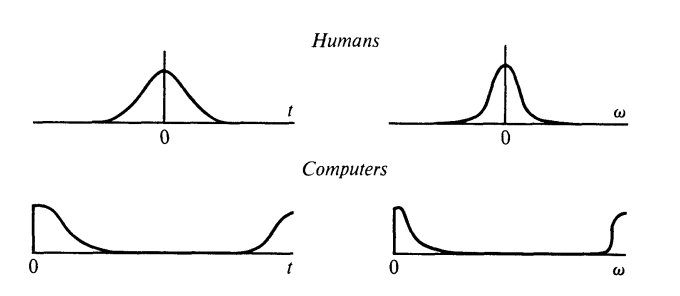
\includegraphics[width=0.5\textwidth]{xrf/human}
\caption[human]{一维傅氏变换程序的计算机内存安排}
\label{fig:xrf/human}
\end{figure}

试考虑对有八个点的时间函数进行一维傅氏变换。位于第一个向量元素的输出是零频
率,代表某一网格的、即函数$+1,-1,+1,
-1\ldots\ldots$的最高频率之Nyquist频率$\pi$是位于该八点
函数的第五个元素,其后伴随以负频率。最小的非零负频率位于第八个向量元素。如杲有第
九个元素,那么它会因周期性之故而等于第一个元素。偏移方法的输出不是实数,是初学者
的常见错误;采用单精度算法
时,虚部应为实部的$10^{-6}$左右,出
现与$1/N$呈正比(N为向量长度)的非常大的虚部,表明有程序错误。

下面是对二维程序的检查程
序,其中,“Write”语句是局部FORTRAN而不是Ratfor语
言。被变换的函数有几分像是时间轴上的某一种低频函数,而更多像是空间坐标轴上的某一种
低频函数。
\begin{minted}{Fortran}
\#Test case for two-dimensional Fourier Transformation

integer it,nt,ix, nx; complex cp(64,64), cwork(64) 
open(4,file= 'plotfile',status= 'new ',access= 'direct',form=
'unformat­ted', reel=l)
nx = 64; nt = 64; do it=l, nt
do ix=l, nx
	do ix=1, nx
		cp(it, ix) = 0.
cp(16,3)=1.; 
cp(16, 4) = 4.; 
cp(16,5)= 6. ; 
cp(16, 6) = 4.; 
cp(16, 7)=1.

cp(17, 3)=1.; 
cp(17, 4) = 4. ; 
cp(17, 5)=6. ; 
cp(17, 6) = 4. ;
cp(17, 7)=1.

call ft2d(nt, nx, cp, +1., +1., cwork)
write(4, rec=l)((real(cp(it, ix)), it=l, nt), ix=l, nx)
stop; end
\end{minted}
最基本的二维傅氏变换如下所示
\begin{minted}{Fortran}
2D Fourier transform by using ID program subroutine
ft2d(nl,n2,cp,signl,sign2,cwork) complex cp(nl,n2),cwork(n2) integer
nl,n2 real signl,sign2}

do i2 = l,n2 # transform over the fast dimension
call fork(nl,cp(l,i2),signl) #one-dimensional Fourier transform
do i 1 = l, n 1 { # transform over the slow dimension
do i2 = 1, n2
cwork(i2) = cp(il,i2)
call fork(n2,cwork,sign2) #one-dimensional Fourier transform
do i2 = l,n2
cp(il ,i2) = cwork(i2)
}
relurn; end

\end{minted}
最后,我们谈一谈一维快速傅氏变换程序。这一个程序是《地球物理数据处理基础》一
书第12页\footnote{中文译本的第19页,见1979年石油化学工业出版社出版之《地球物理数据处理基础》。——译者}上的FORTRAN语言子程序“fork”之Ratfor语言的翻版。照例,lx是2的整数
幂,输出cx(l)是零频率,cx(lx/2+
l)是所谓Nyquist频率,而cx(lx)则是最小负频
率。算法简短又策略,除非你参考其他的资料,你休想读得懂该程序。
\begin{minted}{Fortran}
# ID fast Fourier transform subroutine fork(lx,cx,signi)
complex cx(lx),carg,cexp,cw, ct j= 1 ; k= 1 ; sc = sqrt(l./lx)

do i = l,lx {

if(i<= j) {ct = cx(j) *sc; cx(j) = cx(i) *sc; cx(i) = ct}
m = lx/2

while(j>m) = m = m/2; if(m<l)break}

j = j + m
}
repeat {
istep=2 *k 
do m=l,k {

carg = (0., 1. ) * (3.14159265 *signi * (m-l))/k; cw = cexp(carg) do i =
m,lx,istep
{ct = cw *cx(i + k); cx(i + k)=cx(i)-ct; cx(i) = cx(i) + ct
}
k=istep
} until(k >= lx)
return; end
\end{minted}
傅氏变换既有实部又有虚部,有时二者均需显示。但往往是虛部略而不计,这是因为我们
用的时间函数大多数是在$t=0$
之前就已等于零了,所以,它们的傅氏变换必须满足一定的条
件,即实部与虚部必须是通过Hilbert变换而相互联系。狭义地说,
一个往往看起来像是余弦,
另一个看来像是正弦。因此,观察到实部,总是能
很容易想像出虚部。图\ref{fig:xrf/two-fourier}是检验程序的输出显示。
\begin{figure}[H]
\centering
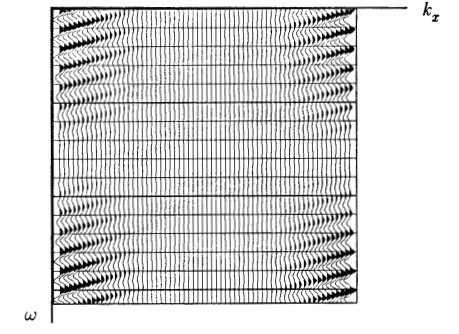
\includegraphics[width=0.5\textwidth]{xrf/two-fourier}
\caption[two-fourier]{二维傅氏变换检验程序的输出}
\label{fig:xrf/two-fourier}
\end{figure}
\subsection{Stolt偏移}
以下所示Stolt偏移程序采用线性内插方法将$\omega$轴转
换为$k_z$轴,用$dk_z/d\omega$进行标定,影响不太大,因而为
使程序简短而将它忽略不计了(对于习题,有些需要保留)。
实例检验的内容是根据脉冲作出半圆波阵面。
\begin{minted}{Fortran}
integer it,nt,ix,nx; real vdtodx; complex cp(256,64)
open(4, file = 'piotfile ',status='new * '.access =' direct
',form = 'unformatted recl = l)
nx = 64; nt = 256; vdtodx= 1./4. #vdtodx = v dt/dx

do it=l,nt
do ix= l, nx

cp(it,ix) = 0.

cp(32,9) = l.; cp(64,17) = 1. ; cp(l28, 33) = 1. 
call stolt(nt, nx, cp, vdtodx)

write(4,rec = l)((real(cp(it,ix)),it = 1, nt), i x = 1,nx)
stop; end

#Stolt migration subroutine without cosine weight.

subroutine stolt(nt,nx,cp,vdtodx)
integer ikx,nx,nt,nth,iktau,iom

real om,vkx,wl,wh,aktau,pi,pionth,vdtodx
complex cp(nt,nx),cbf(l025)

pi = 3. 14159265; nth = nt/2; pionth = pi/nth;

call ft2d(nt,nx,cp, 1. ,-l. ,cbf)

do ikx=l ,nx {

vkx = (ikx-l) * 2 * pi * vdtodx/nx

if(ikx > nx/2)vkx = 2.* pi * vdtodx-vkx #negative k_x

cbf( l) = 0. ; cbf(nt+1 = 0.  # cbf= working buffer

do iom=l,nt

cbf(iom) = cp(iom,ikx) # Omit weighting

cp( 1 ,ikx) = 0. # Ignore zero freq
do iktau = 2,nth+1 { # Stretch
aktau = (iktau-l.0l) *pionth
om = sqrt(aktau * aktau +vkx * vkx) ; iom= 1 +om/pionth
if(iom<nth) {
  wl = iom-om/pionth; wh=l.-wl
  cp(iktau, ikx) = wi * cbf(iom) + wh * cbf(iom +1)
  cp(nt-iktau + 2, ikx) = wl * cbf(nt-iom + 2) + wh * cbf(nt-iom+1)
}
else
cp(iktau, ikx) = 0.
}

call ft2d(nt,nx,cp,-l. , 1. ,cbf) 
return; end
\end{minted}
这种检验程序的输出曾经在1.3节内显宗过,为棱好地阐明解的周期性质,其余一个半
圆波阵面外所有其他均已消除了,而且该输出结果是按非线性增益来显示的。图\ref{fig:omk/stolt4}中逐
端相接出现的是四个相同图形。
\begin{figure}[H]
\centering
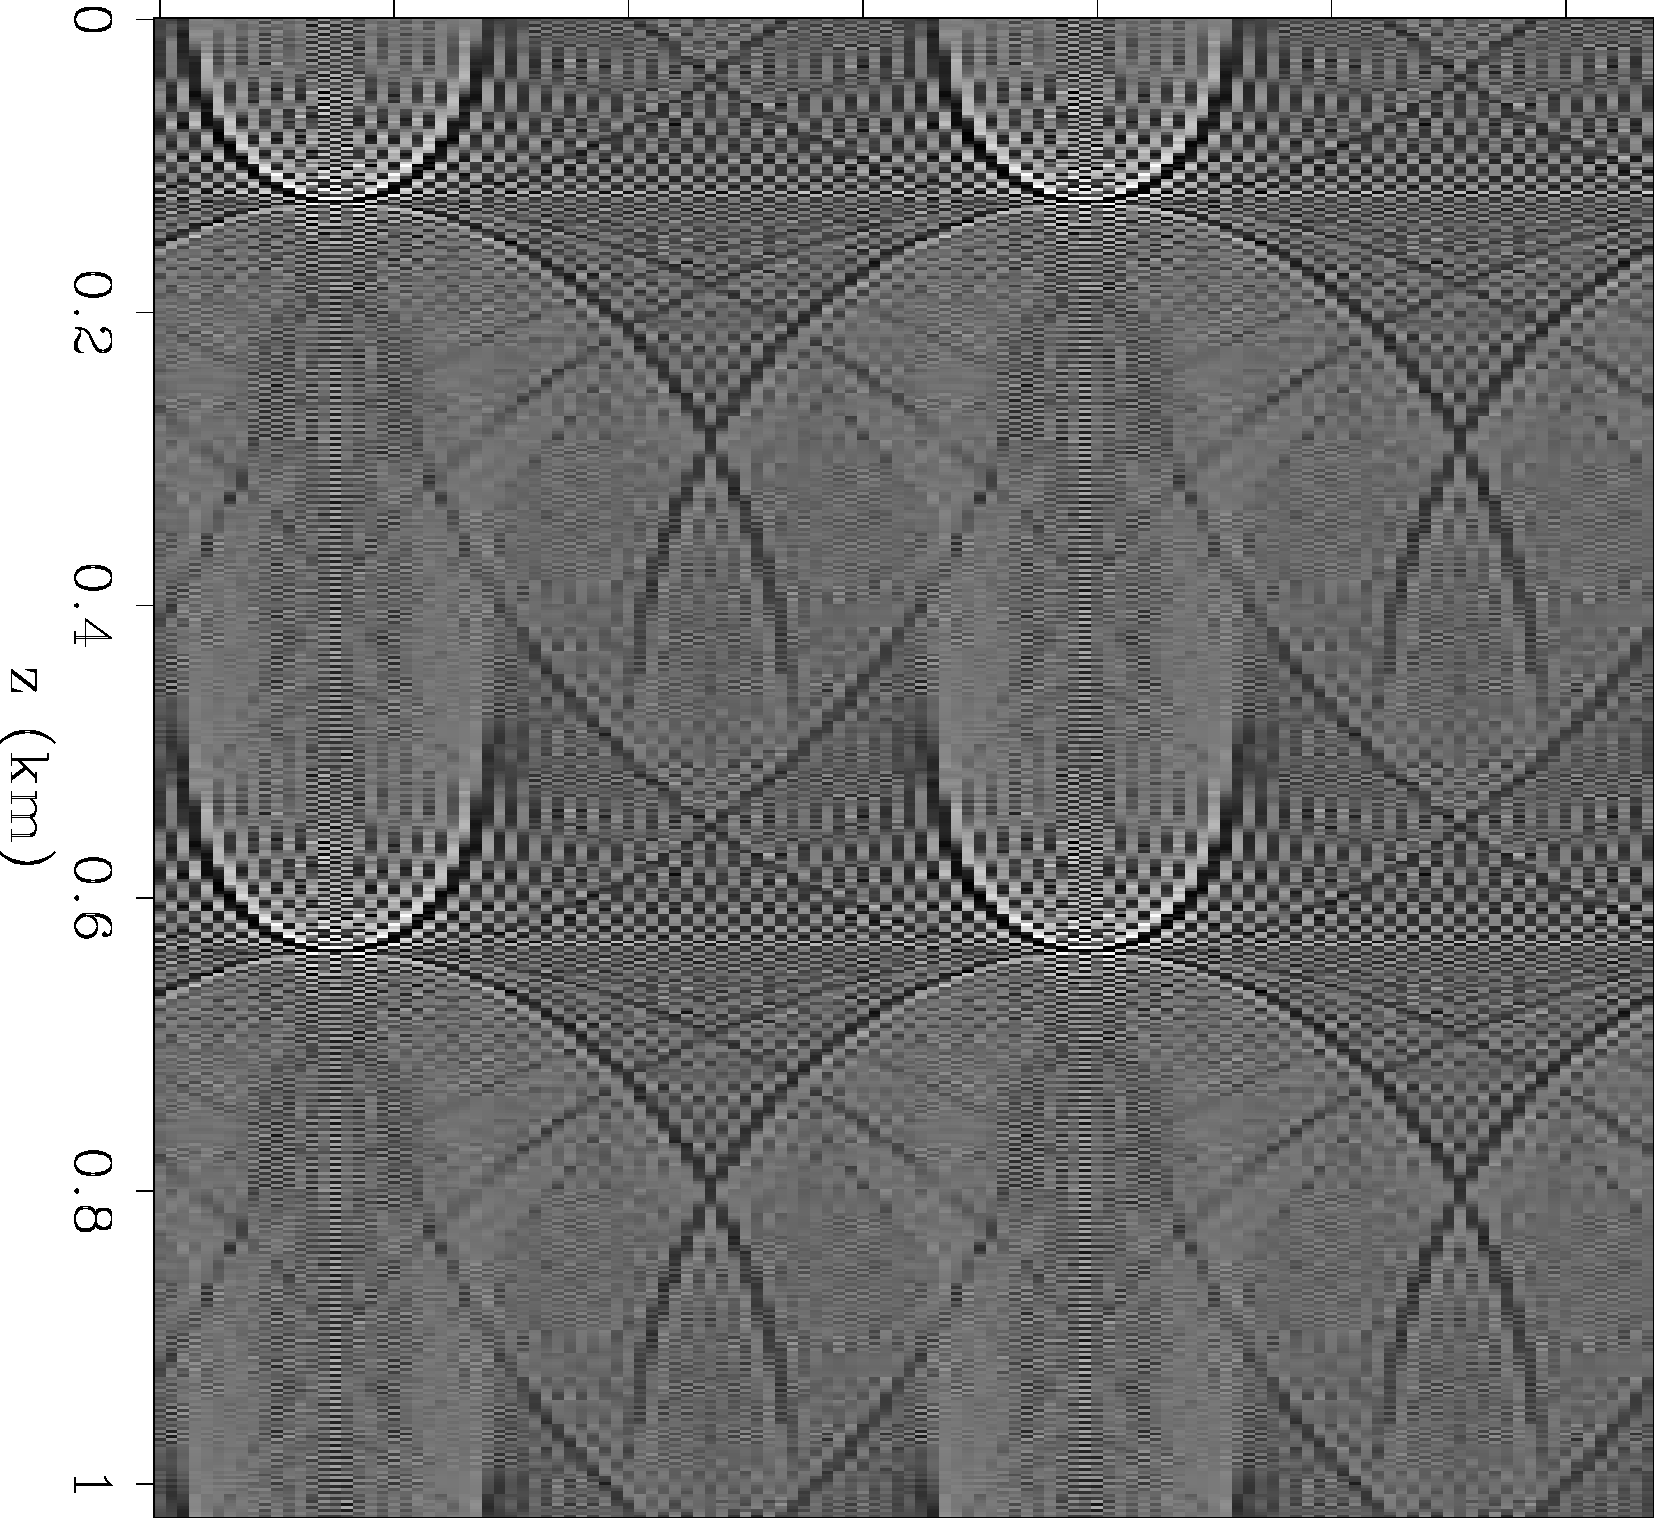
\includegraphics[width=0.5\textwidth]{omk/stolt4}
\caption[stolt4]{Stolt偏移程序输出的周期性}
\label{fig:omk/stolt4}
\end{figure}
\subsection{Rocca的按行傅氏变换}
Rocca的按行傅氏变换比原始程序要快速一点,因为基本的一般性运算是一次完成,而
这时每行均实现了傅氏变换。但是Rocca方法超过原始方法的主要优点在于不需数据的转
置,而且即使在按页读的条件下该程序也能有效地运行。
\begin{minted}{Fortran}
#Try Rocca's row Fourier transform.
# sign2 should be+l.or-l.it is the sign of i. 
subroutine rowcc(nl,n2,cx,sign2,scale) 
complex cx(nl,n2),cmplx,cw,cdel 
do il =l,nl do i2=l,n2
cx(il,i2)= cx(il,i2)* scale
doi = 1,n2 {
if(i <= j) call twidl(nl,cx(l,i),cx(l,j))
m = n2/2
while(j>m) {j = j-m; m = m/2; if(m<1)break}
j = j + m } 
istep = 1
repeat {
istep = 2 * istep; cw = i.
arg=sign2 *3.14159265/istep;} cdel = cmplx(cos(arg),sin(arg))
do m=l,istep {
do i = m,n2,istep
call twid2(n 1, cw, cx( 1, i), cx( 1,i + lstep)) 
cw = cw * cdel
istep = istep } until(istep>=n2) 
return; end

subroutine twidl(n,cx,cy) 
complex cx(n),cy(n),ct
doi=l,n {ct = cx(i); cx(i) = cy(i); cy(i) = ct}
return; end

#If you feel like optimizing,this is the place, 
subroutine twid2(n,cw,cx, cy) 
complex cx(n),cy(n),ctemp,cw
do i = l,n {ctemp = cw*cy(i); cy(i) = cx(i)-ctemp; cx(i) = cx(i)+ ctemp} 
return; end
\end{minted}
\subsection{习 题}
\begin{enumerate}
\item 大多数时间函数均属实函数,其虚部为零。试证:这意味着$F(\omega,k)$可由$F(-\omega,-k)$确定。
\item 利用你的计算机和图形显示仪,试检验图\ref{fig:xrf/two-fourier}是用所给出的程序作出的。

\item 前一题中所显示的傅氏变换之实部有点难以解释,因为负频率与负波数的处置很棘
手。试修正该程序使$F(\omega,k)$的原点位于显示网格的中心(33,33)。提示:在进行傅氏变换之前简单修改$f(t,x)$就行了;回想一下“时移定理”。写出$f(t,x)$和新的更容易
解释的$F(\omega,k)$,标明坐标轴。
\item 时间$t=0$时在地表面位于$x=32$之处的点源爆炸得出的在$(t,x)$平面内之合成观
测结果如下面\ref{fig:dft/airwave}左图所示。右图是$(\omega,k_x)$平面上的二维傅氏变换之量值。每张图的原点位
于各该图的左上角。试问在速度值降低一半的地层中这些图看上去会是什么样子?
\begin{figure}[H]
\centering
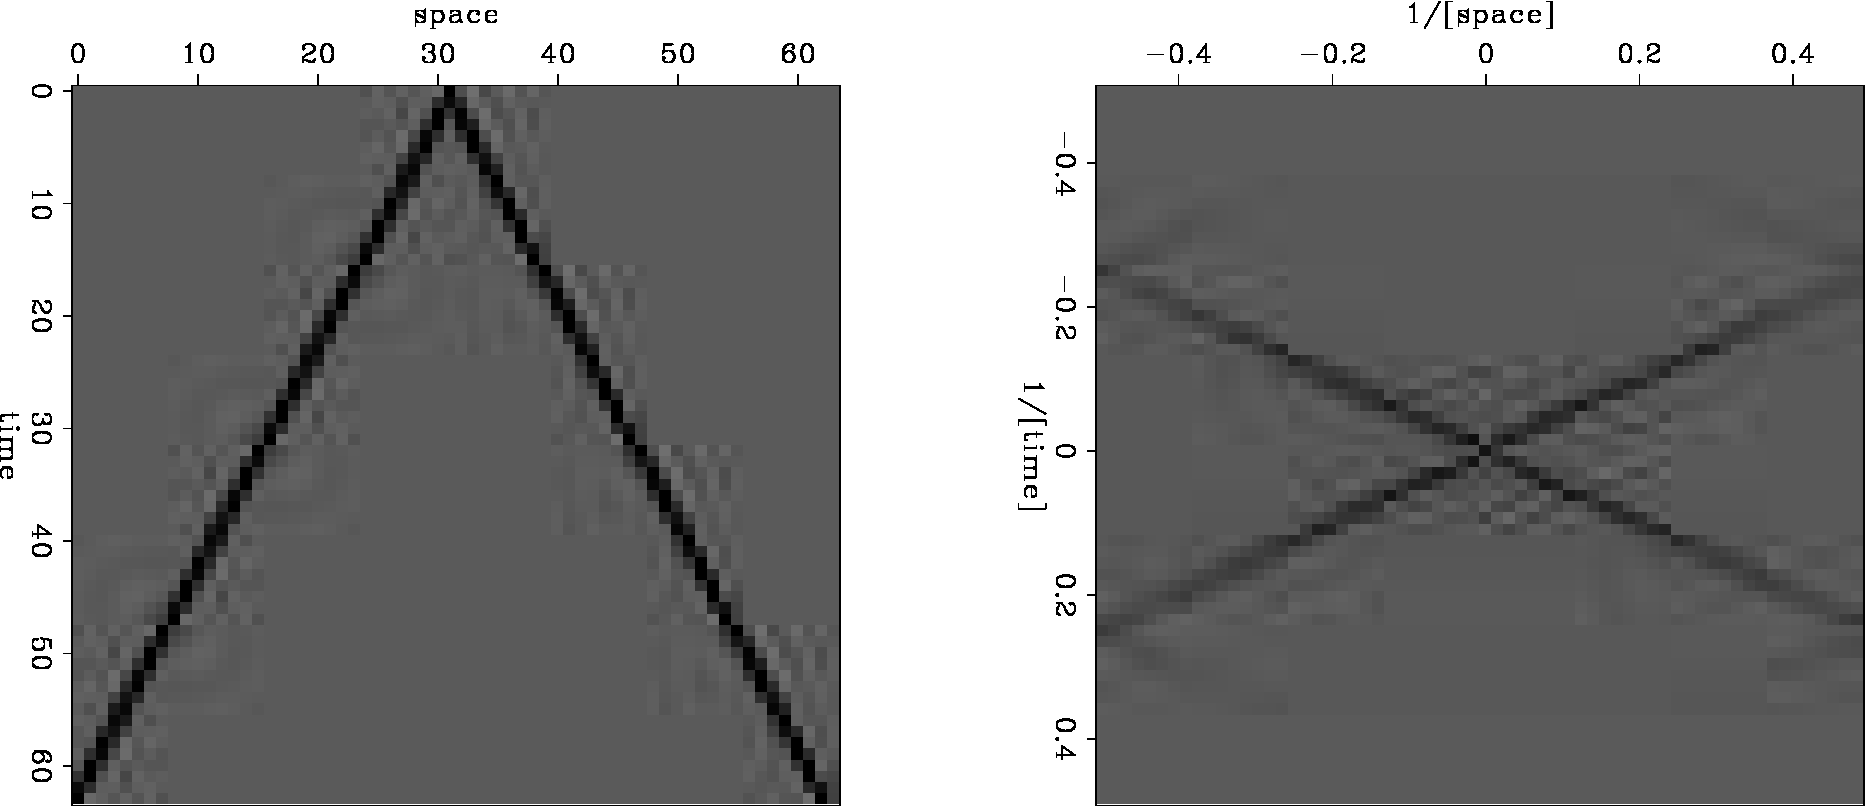
\includegraphics[width=0.95\textwidth]{dft/airwave}
\caption[airwave]{习题4}
\label{fig:dft/airwave}
\end{figure}
\item 在Stolt偏移程序中插入适当的余弦倾斜因子函数。试检验并证明除某种有角度依
赖关系的比例因子之外,差异很小。
\item 根据Stolt方法,写一个绕射程序。就是说,已知地层内的点散射体,试用该程序
作出适当的双曲线。
\item 当你使Stolt绕射程序内包括有余弦加权函数的倒数时,要谨防在尖灭边缘上有极
点存在。试问在加权之前还是在加权之后进行拉伸处理才比较妥当?为什么?
\item 使$P(\omega)$随$\omega$的振荡速率减小就能够减少Stolt程序之内插误差,这么处理时要注意
$p(t)$对于负$t$应等于零。因此,在内插之前用$e^{-i\omega\tau}$乘$P(\omega)$,然后在内插以后又用它来
除。试问:程序中采用的常数$\tau$应取什么合适的值?
\end{enumerate}
